\section{Virtualização}

Segundo os autores \citeonline{jain2016virtualization}, o termo ``virtualização'' pode ser definido como uma abstração dos recursos computacionais. Dessa forma, permite-se que um único recurso físico esteja disponível como múltiplos recursos virtuais ou que múltiplos recursos físicos estejam disponíveis como um único recurso virtual.

Uma das formas de virtualização é através de softwares conhecidos como \textit{Hypervisors}. Os \textit{Hypervisors} podem ser executados diretamente sobre o hardware, possuindo seus próprios \textit{drivers} e, portanto, não necessitando de todo um sistema operacional (SO). Ou, podem ser executados na camada de software, como qualquer outro programa executado pelo computador \cite{eder2016virtualization} \cite{jain2016virtualization}.

Uma outra forma de virtualização, é através do uso de contêineres. Em um sistema operacional, existem algumas características e funcionalidades necessárias para isolar um processo do outro. Softwares de virtualização baseados em contêineres utilizam essas funcionalidades para criar um ambiente isolado para processos, um contêiner. Dessa forma, os contêineres compartilham o \textit{kernel} do sistema do operacional em que estão sendo executados. Por isso, as aplicações devem ser compatíveis com o \textit{kernel} do sistema operacional e a arquitetura da Unidade de Processamento Central (CPU, do inglês \textit{Central Processing Unit}) \cite{eder2016virtualization}.

Na Figura \ref{fig:virtualizacao-camadas-containers-e-hypervisor}, observa-se como os softwares de virtualização baseados em contêineres e \textit{Hypervisors} funcionam. O \textit{Hypervisor} separa os recursos da máquina física (hospedeira) para que eles possam ser particionados e dedicados às máquinas virtuais (convidadas). Já em um contêiner, tem-se apenas a aplicação em um ambiente isolado com todos os elementos necessários para executa-lá \cite{potdar2020docker}.

Os autores \citeonline{potdar2020docker} diferenciam as duas tecnologias de virtualização apontadas anteriormente no texto e apresentam algumas vantagens e desvantagens. A criação de máquinas virtuais através de \textit{Hypervisors} demandam mais recursos (CPU, memória e armazenamento), levam mais tempo para inicializar e a customização das imagens que iniciam as máquinas virtuais é mais difícil. No entanto, apresentam a vantagem de isolar os processos a nível de hardware e fornecer um sistema operacional dentro de cada máquina virtual. Por outro lado, a criação de contêineres demandam menos recursos, levam menos tempo para iniciar e a criação de imagens que iniciam os contêineres é relativamente fácil. Porém, o sistema operacional da máquina é compartilhado pelos contêineres. A utilização de cada tecnologia depende do cenário em que se deseja utilizar e podem até mesmo ser utilizadas em conjunto.

\begin{figure}[ht]
    \centering
    \begin{subfigure}[b]{0.45\textwidth}
        \centering
        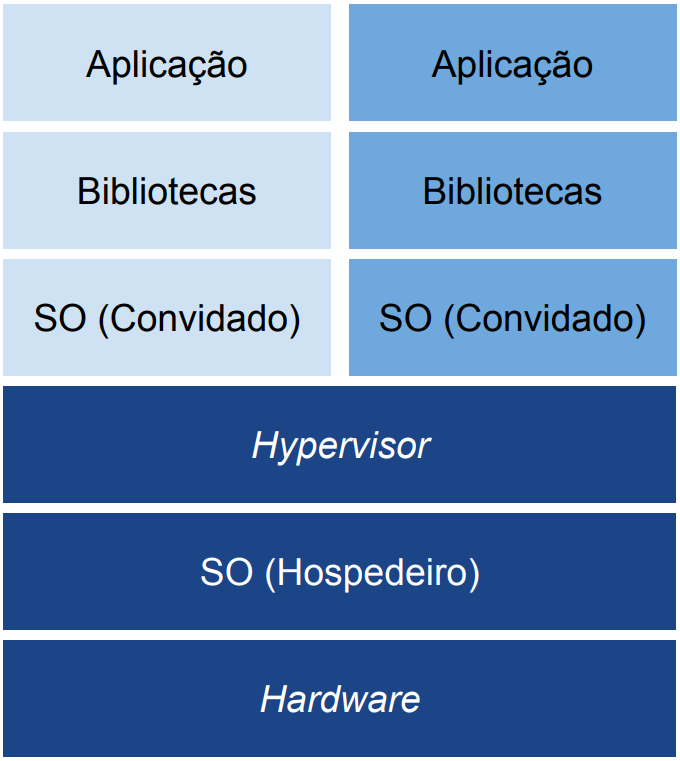
\includegraphics[width=0.8\textwidth]{virtualizacao-hypervisor.png}
        \caption{Máquinas Virtuais.}
        \label{fig:virtualizacao-hypervisor}
    \end{subfigure}
    \hspace{1mm}
    \begin{subfigure}[b]{0.45\textwidth}
        \centering
        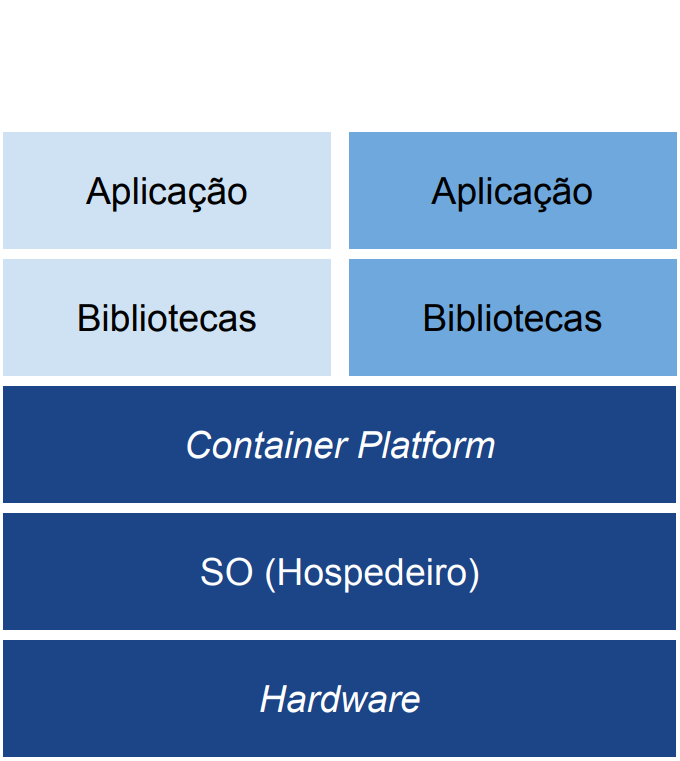
\includegraphics[width=0.8\textwidth]{virtualizacao-containers.png}
        \caption{contêineres.}
        \label{fig:virtualizacao-containers}
    \end{subfigure}
    \caption{Camadas de hardware e software em diferentes soluções de virtualização.}
    \footnotesize Fonte: Produção do próprio autor.
    \label{fig:virtualizacao-camadas-containers-e-hypervisor}
\end{figure}

\section{Computação em nuvem e borda}

Segundo os autores \citeonline{mohammed2021sufficient}, o termo ``computação em nuvem'' pode ser definida como um ambiente na Internet que permite utilizar softwares, dados e recursos de qualquer lugar. Nesse sentido, as tecnologias de virtualização foram essenciais para realização do que hoje entende-se como computação em nuvem. Assim, pode-se caracterizar três tipos básicos de modelos de serviço de computação em nuvem:
\begin{itemize}
    \item \textit{Infrastructure as a Service} (IaaS): o usuário gerencia recursos computacionais (máquinas virtuais, endereços IP, armazenamento, rede, etc).
    \item \textit{Platform as a Service} (PaaS): o usuário gerencia plataformas de computação, permitindo construir aplicações e distribuídas na rede;
    \item \textit{Software as a Service} (SaaS): o usuário tem acesso a aplicações gerenciadas por um provedor. Tais aplicações são disponibilizadas através da Internet, eliminando a necessidade do usuário de instalar softwares em seu computador pessoal.
\end{itemize}

Por outro lado, o termo ``computação em borda'' é um conceito que se refere à estratégia de trazer os serviços e aplicações de computação em nuvem para perto, geograficamente, do usuário final possibilitando um menor tempo de resposta \cite{khan2019edge}. Normalmente, os usuários finais executam as aplicações em dispositivos com capacidade limitada de processamento, o que implica no uso da nuvem para execução dos principais serviços e aplicações. Como resultado, problemas de alta latência e mobilidade são recorrentes.

Segundo os autores \citeonline{khan2019edge}, os problemas de computação em nuvem podem ser resolvidos por diferentes modelos de computação em borda. Um deles é a computação em névoa, que estende os recursos computacionais disponíveis na nuvem para a borda da rede através do uso de vários dispositivos interconectados \cite{coutinho2016nevoa}. No entanto, estender uma plataforma altamente virtualizada para borda da rede é um desafio. Isso, \recom{porqu\^{e},}{porque} envolve o uso de diferentes hardwares, protocolos de rede, grande número de dispositivos, entre outras dificuldades.

\section{Arquitetura de Microsserviços}

Uma aplicação monolítica pode ser caracterizada como um software cujos módulos não podem ser executados de forma independente \cite{dragoni2017microservices}. À medida que a complexidade da aplicação cresce, torna-se difícil realizar manutenção e localizar problemas. Além disso, uma pequena mudança em um dos seus módulos resulta na necessidade de reinicialização de toda a aplicação.

Nesse contexto, arquiteturas de microsserviços têm sido propostas como solução para os problemas encontrados em aplicações monolíticas. Segundo os autores \citeonline{dragoni2017microservices}, um microsserviço é um processo coeso e independente que interage com outros microsservicos por meio de mensagens. Nessa definição, utiliza-se o termo ``coeso'' para indicar que cada microsserviço implementa apenas funcionalidades fortemente relacionadas ao que ele realiza. Assim, uma arquitetura de microsserviços pode ser definida como uma aplicação distribuída \add{(Você não definiu o que seria uma aplicação distribuída. Talvez fosse interessante trazer a definição no primeiro parágrafo, contrapondo a definição de aplicação monolítica.)} onde todos os módulos são microsserviços. Esse tipo arquitetura de desenvolvimento tornou-se amplamente utilizada pela indústria ao possibilitar alta disponibilidade, flexibilidade, escalabilidade e velocidade. Como cada microsserviço é um processo independente, pode ser escalado conforme a necessidade, diferentemente de uma arquitetura monolítica onde seria necessário escalar todos os módulos.


\section{Kubernetes}

Kubernetes é uma plataforma \add{de} código aberto, portável e extensiva para o gerenciamento de cargas de trabalho e serviços distribuídos em contêineres \cite{google2023kubernetes}. Um \textit{cluster} Kubernetes pode ser caracterizado como um conjunto de servidores de processamento, nós, responsáveis por executar os contêineres. 

Obrigatoriamente, em um \textit{cluster}, deve existir um plano de controle a ser executado em um dos nós ou replicado em diversos. O plano de controle é responsável por gerenciar o \textit{cluster}, decidir onde alocar as aplicações, responder a eventos, etc. Os seus principais componentes são: (i) \textit{kube-apiserver}, uma API (do inglês, \textit{Application Programmable Interface}) que expõe as funcionalidades do \textit{cluster}; (ii) \textit{etcd}, um banco de dados distribuído para armazenar o estado do \textit{cluster}; (iii) \textit{kube-scheduler}, aplicação responsável por decidir em que nó cada unidade básica de escalonamento será alocada dentro do \textit{cluster}, levando com conta os recursos e restrições impostas; (iv) \textit{kube-controller-manager}, componente com os diversos controladores do \textit{cluster}.

Além disso, em todos os nós, é necessário que algumas aplicações sejam executadas para que sejam controlados pelo plano de controle. Esses componentes são: (i) \textit{kubelet}, aplicação que garante a execução dos \recom{\textit{containers}}{contêineres}; e (ii) \textit{kube-proxy}, \textit{proxy} de rede executado em cada nó que realiza o encaminhamento de trafégo de rede corretamente dentro do \textit{cluster}. Na Figura \ref{fig:kubernetes-componentes}, observa-se como esses componentes se integram e formam um \textit{cluster} para o gerenciamento de cargas de trabalho e serviços distribuídos.

\add{Em nenhum lugar está descrito \textit{kubectl} que aparece na figura. Você acha que seria interessante fazer isso?}

\begin{figure}[ht]
    \centering
    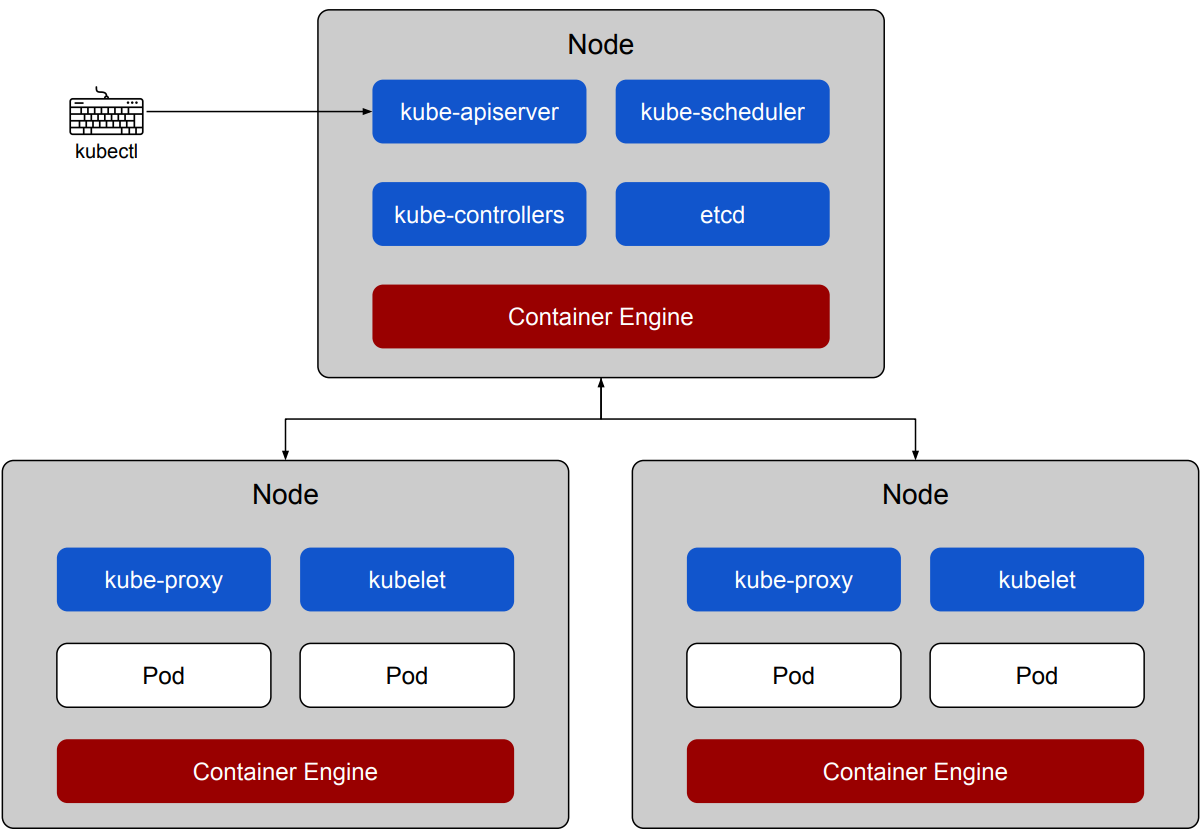
\includegraphics[width = 0.75\textwidth]{k8s-components.png}
    \caption{Componentes de um \textit{cluster} Kubernetes.}
    \footnotesize Fonte: Produção do próprio autor.
    \label{fig:kubernetes-componentes}
\end{figure}

Através da API disponibilizada pelo plano de controle, diversos recursos estão disponíveis para criação. Estes recursos podem ser entendidos como objetos ou entidades persistentes. Uma vez criado, os componentes do \textit{cluster} trabalham para garantir a sua existência. Dentre eles, tem-se:
\begin{itemize}
    \item \textit{Pod}: é o recurso mais simples, a unidade básica de um \textit{cluster} Kubernetes, e pode conter um ou mais contêineres;
    \item \textit{ReplicaSet}: recurso que garante que um número de réplicas de um determinado \textit{Pod} esteja em execução;
    \item \textit{DaemonSet}: recurso que garante um \textit{Pod} executando em cada nó do \textit{cluster};
    \item \textit{Job}: recurso que garante que um ou mais \textit{Pods} sejam executados com sucesso.
\end{itemize}

Para cada recurso, é necessário um controlador associado para garantir que o estado desejado seja alcançado. Além dos recursos disponíveis por padrão, a API do Kubernetes também permite a criação de recursos customizados. No entanto, pode ser necessário o desenvolvimento de um controlador associado para implementar a lógica de controle.

\section{Espaços Inteligentes Programáveis}

Segundo o autor \citeonline{carmo2021arquitetura}, um Espaço Inteligente é definido como um espaço físico equipado com uma rede de sensores, atuadores e serviços computacionais que atuam com o objetivo de atender as necessidades dos usuários presentes no ambiente. Além disso, o autor aponta que esses elementos devem ser gerenciados por uma infraestrutura de hardware e software responsável por coletar e analisar os dados, gerar decisões e atuar quando necessário. Para isso, uma arquitetura baseada em microsserviços com orquestração multinível centrada na observabilidade e programabilidade granular da infraestrutura é proposta, um Espaço Inteligente Programável (PIS, do inglês \textit{Programmable Intelligent Space}).

\subsection{Arquitetura}

A arquitetura proposta por \citeonline{carmo2021arquitetura} possui 4 camadas horizontais e 2 camadas transversais. Na Figura \ref{fig:pis-model-conceitual}, pode-se observar todas camadas, suas principais funções e como se relacionam.

\begin{figure}[ht]
    \centering
    \includegraphics[width= 125mm]{PIS-model.png}
    \caption{Modelo Conceitual da arquitetura do PIS.}
    \footnotesize Fonte: \citeonline{carmo2021arquitetura}
    \label{fig:pis-model-conceitual}
\end{figure}

A camada de virtualização é responsável por abstrair os recursos de hardware e torná-los disponíveis para o uso. Nesse sentido, utilizam-se softwares como \textit{Hypervisors} e plataformas de criação de contêineres nessa camada. Superior à camada de virtualização, a camada de comunicação é responsável por fornecer conectividade e interação entre as aplicações. As aplicações podem utilizar diferentes protocolos dentro do PIS, tais como HTTP (do inglês, \textit{Hypertext Transfer Protocol}) ou AMQP (do inglês, \textit{Advanced Message Queuing Protocol}). Na Seção \ref{sec:pis-comunicacao}, os detalhes de cada protocolo de comunicação são explorados.

A camada de serviços engloba as aplicações desenvolvidas, enquanto a camada de suporte à aplicação \recom{trata-se das}{corresponde às} bibliotecas e ferramentas auxiliares para o desenvolvimento delas. Já a camada de segurança tem como responsabilidade realizar controle de acesso, segurança dos dados, segurança da comunicação e gerenciamento de privacidade. Por isso, \add{essa última está} presente ao longo de todas as \recom{4}{quatro} camadas horizontais.

Por fim, tem-se a camada de gerenciamento, responsável por gerenciar os elementos de todas as \recom{4}{quatro} camadas horizontais. Para isso, deve prover as seguintes funções: (i) Orquestração e Informações multinível; (ii) Observabilidade; e (iii) Gerenciamento dos recursos. 

% \begin{itemize}

%     \item Orquestração e Informações multinível: a orquestração pode ser realizada através de \textit{softwares} como Kubernetes, que permite a alocação de contêineres em um conjunto de máquinas através de diversas estratégias. 
    
%     \item Observabilidade: pode ser definido como a capacidade de visualizar e compreender o comportamento de um sistema reunindo, processando dados do sistema e apresentando os de maneira adequada \cite{picoreti2018observability}. Aplicações podem ser implantadas em \textit{clusters} Kubernetes para permitir a coleta de métricas, \textit{logs}, rastreios. \textit{Softwares} como Prometheus, um servidor de métricas, pode ser instalado e configurado para coleta de diversas métricas do sistema (uso de CPU, memória, disco, etc). Além disso, para analisar o desempenho do sistema pode-se utilizar funções de rastreamento através da instrumentação do código e sistemas de coleta dessas informações, tais como Zipkin. Na seção \ref{sec:pis-rastreamento}, os detalhes sobre rastreamento são explorados.

%     \item Gerenciamento de recursos: através do próprio Kubernetes pode-se gerenciar os recursos que estão sendo orquestrados. Além disso, também pode-se utilizar \textit{softwares} como OpenStack para criação de máquinas virtuais.

% \end{itemize}


\subsection{Comunicação}
\label{sec:pis-comunicacao}

O protocolo HTTP é um protocolo de comunicação na camada de aplicação do modelo OSI (do inglês, \textit{Open System Interconnection}) amplamente utilizado e difundido. É baseado no padrão cliente/servidor, onde um servidor é um programa responsável por aceitar conexões de requisições de serviço e enviar respostas. Por outro lado, um cliente é uma aplicação que estabelece conexões com o servidor com o objetivo de enviar requisições \cite{berners1996hypertext}.  No contexto do protocolo HTTP, há oito tipos de requisições (também chamados de métodos HTTP) que o cliente pode iniciar. Assim, o servidor responde adequadamente a cada uma dessas requisições com um código de três dígitos informando ao cliente o \textit{status} da solicitação. A seguir, tem-se os principais métodos e as ações que realizam:

\begin{itemize}
    \item GET: usado para ler informações do servidor;
    \item PUT: usado para modificar completamente um dado no servidor ou gerar um novo dado nele;
    \item POST: usado para transferir dados ao servidor, na forma de arquivos, formulários ou outros;
    \item DELETE: usado para remover um dado especificado no servidor.
\end{itemize}

O protocolo AMQP também é um protocolo de comunicação na camada de aplicação do Modelo OSI. No entanto, é um protocolo de comunicação assíncrono orientado a mensagens baseado no padrão \textit{publish}/\textit{subscribe}. Como apontado pelos autores \citeonline{eugster2003pusub}, no padrão \textit{publish}/\textit{subscribe}, os produtores publicam mensagens em um barramento, enquanto os consumidores se subscrevem para receber mensagens com as informações que desejam. 

% NÃO SEI SE VOU DEIXAR ISSO
% Além disso, os autores \citeonline{eugster2003pusub} destacam que comunicações ponto-a-ponto e síncronas levam a aplicações rígidas e estáticas, fazendo com que a escalabilidade do sistema seja prejudicada.

A utilização do protocolo AMQP está associada à execução de uma aplicação conhecida como \textit{broker}, responsável por realizar o roteamento das mensagens dos produtores para os consumidores corretamente. Se necessário, também pode armazenar as mensagens para entregar aos consumidores quando estes estiverem disponíveis.

% O autor \citeonline{queiroz2016infraestruturaespaco} detalha o roteamento de mensagens dentro do PIS através do \citeonline{rabbitmq2023rabbitmq} como  \textit{broker}. Para implementar o padrão de comunicação \textit{publish}/\textit{subscribe}, \citeonline{rabbitmq2023rabbitmq} cria filas  para armazenar as mensagens. No entanto, apenas as filas não são suficiente. É necessário um elemento de roteamento das mensagens responsável por encaminhar corretamente cada mensagem à fila correta. Este elemento, é denominado \textit{exchange}. Além disso, a relação entre uma fila e uma \textit{exchange} é denominada \textit{binding} e podem ser entendida como uma regra de roteamento. Quando uma mensagem é enviada, esta deve possuir uma \textit{exchange} de destino. Bem como, sua identificação de roteamento, denominada \textit{routing key}.

% \begin{figure}[ht]
%     \centering
%     \includegraphics[width = 0.5\textwidth]{img/roteamento-multiplas-filas.png}
%     \caption{Representação da comunicação entre um produtor e dois consumidores, com um \textit{exchange}, duas filas e três diferentes \textit{bindings}}
%     \footnotesize Fonte: \citeonline{queiroz2016infraestruturaespaco}.
%     \label{fig:roteamento-multiplas-filas}
% \end{figure}

% Considere a Figura \ref{fig:roteamento-multiplas-filas}, que o autor \citeonline{queiroz2016infraestruturaespaco} aponta como exemplo. O produtor, P1, envia as mensagens à \textit{exchange} X1. Os consumidores C1 e C2 possuem as suas filas associadas, respectivamente, Q1 e Q2 . Observe que, a fila Q1 possui um \textit{binding}, B1, com a \textit{exchange} X1. Enquanto, a fila Q2 possui dois \textit{bindings}, B1 e B2, com a \textit{exchange} X1. Assim, se uma mensagem for enviada ao \textit{broker} com a \textit{exchange} X1 de destino e \textit{routing key} B1, ambas as filas Q1 e Q2 irão receber a mensagem. No entanto, se uma mensagem for enviada ao \textit{broker} com a \textit{exchange} X1 de destino e \textit{routing key} B2, apenas a fila Q2 irá receber a mensagem.

% Existem diversas categorias de \textit{exchanges}, a mencionada no exemplo anterior é do tipo \textit{direct}. Onde, a mensagem é encaminhada para a fila de acordo com o \textit{binding}. No entanto, este tipo de \textit{exchange} possui limitações. Para realizar um roteamento de mensagens baseados em múltiplos critérios, uma \textit{exchange} do tipo \textit{topic} deve ser utilizada. Nesse tipo de \textit{exchange}, mensagens enviadas ao \textit{broker} não podem ter uma \textit{routing key} arbitrária - deve ser uma lista de palavras separadas por pontos.

% Assim, na camada de comunicação do PIS são utilizadas \textit{exchanges} do tipo \textit{topic} para permitir uma maior flexibilidade de roteamento das mensagens ao construir um lista de palavras com tipos e subtipos, tais como \textit{CameraGateway.0.Frame}. A primeira palavra representa o serviço, a segunda o identificador da câmera e a terceira o tipo de informação da câmera, no caso uma imagem. Para receber imagens de todas as câmeras que enviam mensagem a \textit{exchange}, basta se subscrever com a seguinte regra: \textit{CameraGateway.*.Frame}.

\subsection{Observabilidade}
\label{sec:observabilidade}

O termo ``observabilidade'' pode ser definido como a capacidade de visualizar e compreender o comportamento de um sistema através da coleta e processamento de dados \cite{picoreti2018observability}. São utilizados três tipos de dados principais para prover informações de observabilidade de um sistema: \textit{logs}, métricas e \textit{traces}.

Os \textit{logs} são linhas de texto estruturadas e não estruturadas que um sistema gera quando uma parte específica do código é executada. Em outras palavras, um \textit{log} é um registro de um evento em um aplicação. Geralmente, são coletados por uma camada de agregação para ser pré-processado e, em seguida, persistido para posterior processamento e análise. Por isso, os \textit{logs} são comumente utilizados para descobrir problemas e analisar comportamentos imprevisíveis do sistema.

Por outro lado, as métricas podem ser definidas como números coletados periodicamente formando uma série temporal. Dessa forma, ajudam a mostrar tendências sobre o comportamento e performance do sistema ao longo do tempo. Para isso, também são coletadas por uma camada de agregação periodicamente para processamento e persistência.

Já os \textit{traces} podem ser entendidos como uma forma de observabilidade do sistema que permite determinar a causalidade entre eventos de diversos aplicações, bem como extrair medidas de desempenho. Para isso, cada serviço deve contribuir propagando um contexto, que deve ser enviado diretamente a uma ferramenta responsável por correlacionar cadeia de eventos e apresentar aos usuários. Na Figura \ref{fig:exemplo-trace}, tem-se um exemplo de \textit{trace} e sua respectiva árvore de \textit{spans} (unidade básica de trabalho, um registo temporal com início e fim associado a alguma função ou serviço) indicando a causalidade entre eles.

\begin{figure}[ht]
    \centering
    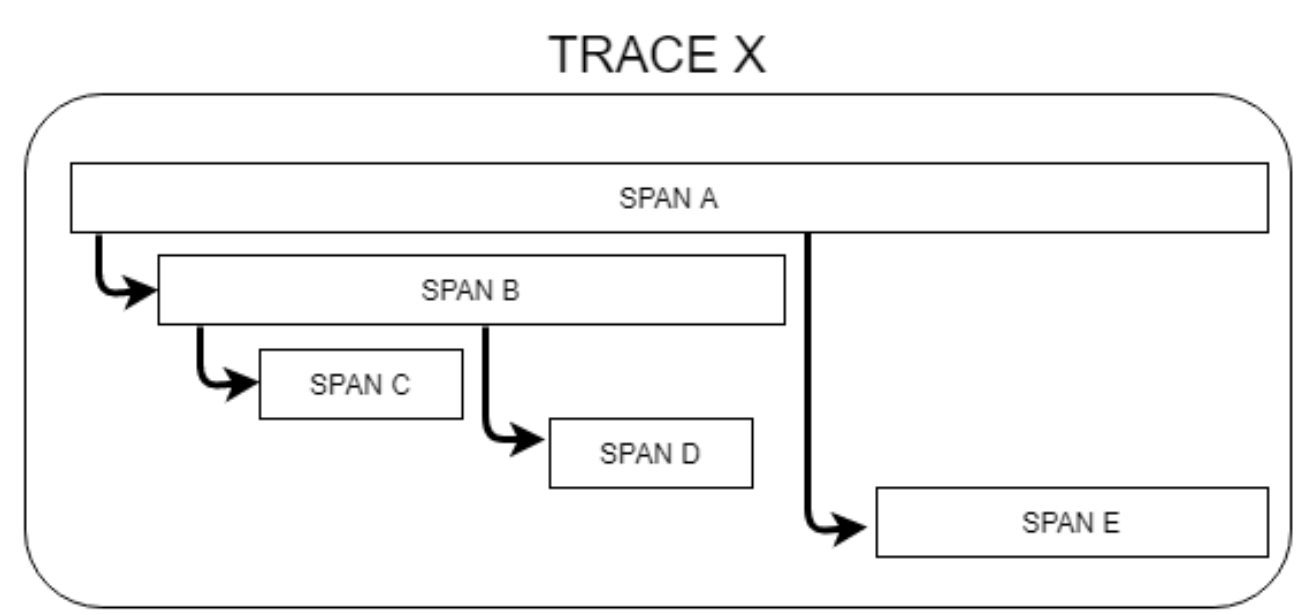
\includegraphics[width=0.5\textwidth]{images/exemplo-trace.png}
    \caption{Exemplo de rastreamento.}
    \footnotesize Fonte: \citeonline{cotta2020medicao}.
    \label{fig:exemplo-trace}
\end{figure}

Por ser um método baseado em anotações, nesse tipo de solução há necessidade de instrumentação do código. Ou seja, é necessário informar no código onde a medição começa e termina \cite{sigelman2010tracing}.

% Assim, em um sistema de rastreamento tem-se \cite{cotta2020medicao} \cite{sigelman2010tracing}:

% \begin{itemize}
%     \item \textit{Annotations}: unidade básica de informação. Pode ser do tipo \textit{timing}, com medições de tempo, ou do tipo \textit{tags} com informações gerais na forma de chaves e valores.
%     \item \textit{Spans}: unidade básica de trabalho, um registo temporal com início e fim associado a alguma função ou serviço. Ou seja, um conjunto de \textit{annotations} do tipo \textit{tags} (para identificar a medição) e \textit{timing} (para medir o tempo decorrido).
%     \item \textit{Trace}: é uma coleção de \textit{spans} na forma de uma árvore, onde os nós representam os \textit{spans} e as arestas representam a relação de causalidade.
% \end{itemize}

% Uma vez realizada a instrumentação do código, os tempos de processamento podem ser observados consultando na interface do Zipkin. Através do trabalho desenvolvido pelo o autor \citeonline{cotta2020medicao}, pode-se obter os tempos de comunicação entre as aplicações através de modificações na camada que implementa a comunicação no PIS. No entanto, para que isso seja possível é necessário configurar corretamente uma ferramenta de sincronização de relógios. Por isso, todos os servidores e dispositivos robóticos serão configurados através da ferramente Chrony, que implementa a sincronização de relógios de diferentes dispositivos através do protocolo NTP.


% \subsection{Processo de orquestração}

% \begin{figure}[ht]
%     \centering
%     \includegraphics[width= 125mm]{img/PIS_orquestracao.png}
%     \caption{Processo de orquestração do PIS.}
%     \footnotesize Fonte: \citeonline{carmo2021arquitetura}
%     \label{fig:pis-orquestracao}
% \end{figure}


\section{Trabalhos relacionados}

 No trabalho proposto pelos autores \citeonline{santoro2017foggy}, uma plataforma de orquestração de aplicações para computação em borda é proposta. De acordo com os requisitos impostos durante o momento de instalação das aplicações, estas eram direcionadas de forma à atender os requisitos geográficos ou de capacidade da rede. Assim, era possível orquestrar aplicações tanto em nuvem quanto em borda (o mais próximo do cliente). Além disso, uma aplicação de detecção facial é apresentada no contexto de cidades inteligentes e alguns cenários são explorados. Ao orquestrar a aplicação de detecção facial perto do cliente, há uma diminuição da largura de banda utilizada na conexão com a nuvem e um menor tempo de resposta. No entanto, os autores não apontam o uso de ferramentas de observabilidade, que poderiam ser utilizadas para atualizar a instalação dessas aplicações na plataforma dinamicamente. Também não é abordado no artigo aspectos relevantes de como a comunicação ocorre, por exemplo, se é um modelo de comunicação baseado em mensagens.

Já no trabalho proposto pelos autores \citeonline{mohamed2017uavfog}, uma plataforma de computação em borda baseada no uso de VANTs para aplicações IoT é proposta. Um VANT equipado com os recursos de computação pode viajar para um local específico quando necessário e permanecer nesse local para oferecer suporte aos aplicativos IoT locais. Cada VANT possui um \textit{broker} com um conjunto de aplicações disponíveis. Assim, caso o serviço desejado pela aplicação IoT local não esteja disponível a bordo, a aplicação pode solicitar à um \textit{broker} em nuvem através do próprio dispositivo. Nesse contexto, os autores mostram que ao colocar aplicações no VANT responde-se de forma mais rápida às requisições ao eliminar a necessidade de consulta em nuvem. No entanto, os autores também não exploram ferramentas \recom{uso}{de} observabilidade e como essas poderiam ser utilizadas dentro da plataforma proposta para uma orquestração inteligente dessas aplicações (em nuvem ou a bordo do VANT).

Um outro trabalho que propõe o uso de VANTs no contexto de computação em borda, foi proposto pelos autores \citeonline{sanchez2021uav}. O objetivo é gerenciar as operações de VANTs remotamente e prover conectividade aos dispositivos locais. Para isso, esses dispositivos robóticos são capazes de prover uma rede 4G e assim disponibilizar conectividade aos dispositivos IoT locais. Também foi proposta a integração nos VANTs de uma plataforma de virtualização de contêineres para a implantação dos serviços necessários. Assim, algumas aplicações são orquestradas a bordo e outras em nuvem. No entanto, os autores não exploram o uso de ferramentas de observabilidade e possibilidade de realizar algum processamento a bordo para execução de tarefas (por exemplo, seguimento de padrões). A plataforma no dispositivo robótico funciona como uma ponte para nuvem, que é responsável por controlá-lo.

O conceito de observabilidade multinível \add{em Espaços Inteligentes} foi introduzido pelo trabalho proposto pelos autores \citeonline{picoreti2018observability}, considerando métricas tanto da infraestrutura quanto das aplicações para melhorar o escalonamento e orquestração automática de aplicações em ambientes de nuvem. Os autores obtiveram melhores resultados com o uso de métricas como tempo de resposta, medido pela aplicação, do que com a utilização de métricas como taxa de utilização de CPU. Além do uso de métricas para o escalonamento, foi apontado como trabalhos futuros \recom{pelos}{por} \citeonline{picoreti2018observability} o uso de \textit{traces} para a identificação de gargalos no sistema e escalonamento das aplicações como forma de mitigação de problemas relacionados à alta latência. Assim, os autores \citeonline{tzanettis2022fusion} proposeram um \textit{framework} de orquestração baseado nos 3 pilares da observabilidade: métricas, \textit{traces} e \textit{logs}. Ao levar em conta tanto as métricas quanto os \textit{traces}, o \textit{framework} de observabilidade é capaz de responder a problemas de latência e escalonar os serviços adequadamente. 

Nesse sentido, o presente trabalho visa estender a plataforma de orquestração de contêineres para os dispositivos robóticos permitindo a computação em borda de aplicações, tal como realizado pelos trabalhos propostos pelos autores \citeonline{santoro2017foggy},  \citeonline{mohamed2017uavfog} e \citeonline{sanchez2021uav}, \recom{e tambem}{assim como} a expansão da abrangência do Espaço Inteligente através dos sensores embarcados. No entanto, \recom{se difere ao }{sua principal diferença está no fato de} utilizar as informações multinível, disponibilizadas pelos serviços que fazem parte do PIS, para gerenciar onde devem ser orquestrados, em nuvem ou em borda, a fim de atender os requisitos das aplicações com utilização racional dos recursos de infraestrutura. Diferentemente dos trabalhos propostos por \citeonline{picoreti2018observability} e \citeonline{tzanettis2022fusion}, nesse trabalho não se pretende utilizar as informações multinível para escalonamento, mas para a correta alocação em nuvem ou em borda. Para validação, pretende-se utilizar uma aplicação de detecção de marcadores visuais e controlar a sua orquestração de acordo com o tempo de resposta.


% atender os requisitos da aplicação com utilização racional dos recursos computacionais
% colocar cenário de expansão da abragencia do PIS também neste paragráfio, deixar a parte do cenário bem claro

% ultima frase: para validação...

% Nesse sentido, o presente trabalho visa estender a plataforma de orquestração de contêineres para os dispositivos robóticos permitindo à computação em borda de aplicações, tal como realizado pelos trabalhos relacionados apresentados anteriormente. No entanto, se difere ao utilizar as informações multinível disponibilizadas pelos serviços que fazem parte do PIS para gerenciar onde devem ser orquestrados, em nuvem ou em borda, a fim de garantir alta disponibilidade para os sistemas com utilização racional dos recursos de infraestrutura. Observe que, no caso aqui apresentado neste trabalho, não basta utilizar métricas de infraestrutura como uso de CPU e memória. Faz-se necessário orquestrar de acordo com métricas características da aplicação, como o tempo de resposta total.

